\documentclass[a4paper,10pt]{article}

%======================================================================
%	Bearbeitung sowohl mit LaTeX als auch mit pdfLaTeX ermoeglichen
%======================================================================
\usepackage{ifpdf}

%======================================================================
%	Verwendete Pakete
%======================================================================
% set language for sorting, hyphenation, sections etc.
\usepackage[ngerman,american]{babel}		% american ist default

%% Latex mit deutschen Umlauten:
%% http://www.cs.albany.edu/~herrmann/latex_umlaute/
%\usepackage[latin1]{inputenc}   % direkte Eingabe von ü,ö,ä,ß in Tex-Source-File erlaubt (statt "a, "o etc.)

\usepackage[utf8]{inputenc}

\usepackage[T1]{fontenc}				% EC-Schriften verwenden (vs. DC) da 8-Bit
				% EC-Schriften als T1-kodierten CM-Schriften
				% European/Ext.-Computer-Modern-(EC)-Schriften
				% Umlaute, Anführungszeichen ...
				% => Umlaute koennen von Latex richtig getrennt werden
				% FAQ 5.3.2
								
\usepackage{ae,aecompl}		% virtuelle-CM-Fonts
				% da EC nicht als PostScript-(Type-1) verfuegbar
				% => keine echten Umlaute in PDF-Dokumenten,
				% sondern nur ``a'' mit zwei Punkten als Extrazeichen drüber 
				%(Problem bei Suche im PDF Viewer).
				% Das ae-Package ermöglicht wieder die korrekte 
				% Suche.
				% By loading the ae package (\usepackage{ae}), 
				% you loose some characters as mentioned in 
				% README. 
				% The package aecompl by Denis Roegel restores
				% these characters which are taken from the ec 
				% fonts. If you use pdftex, you will get these 
				% characters as bitmaps, but this might be 
				% better than not having them at all.


%\usepackage{times, mathptm}	% TimesNewRoman Schrift (Acrobat Reader Fonts), 
				% dazu braucht man auch den entsprechenden 
				% Zeichensatz für den Math-Mode
%\usepackage{pslatex}		% ? mathematische Formeln mit Standard 
												% Postscript Fonts gesetzt
				% Paket     Roman         Serifenlos  Typewriter
				% -----------------------------------------------
				% times     Times         Helvetica   Courier
				% palatino  Palatino      Helvetica   Courier
				% newcent   NewCenturySch AvantGarde  Courier
				% bookman   Bookman       AvantGarde  Courier
				% Diese Schriften sind die Standard-PostScript-Schriften
				% und in jedem Drucker verfügbar

\usepackage{
%	german,			% Deutsche Trennungen (ALTE Rechtschreibung), 
							% Anführungsstriche und mehr 
%	ngerman,		% Deutsche Trennungen (NEUE Rechtschreibung), 
							% Anführungsstriche und mehr
							%
%	acronym,		% Verwaltung von Abkuerzungen
%	bibgerm,		% Deutsche Bibliographie, z.B. für package gerapali (German APA-like)
	calc,				% Erweiterung der arithmetischen Funktionen in LaTeX
							% wird verwendet um Titelseite zu zentrieren
	color,			% im Laufenden Text einfach mit \color{Farbe) zwischen den 
							% Farben umschalten, wobei Farbe einfach 
							% durch z.B. red, blue, black etc. ersetzt wird
							% \textcolor{farbe){Text)
%	epigraph,		% Zitat am Kapitelanfang
%	fancyhdr,		% Kopf- und Fußzeilen von Dokumenten frei 
							% gestalten (ähnlich scrpage2)
%	fancybox,		% shadowbox, doublebox, ovalbox, Ovalbox 
%	fancyvrb,		% verbatim Erweiterung:
	float,			% Positionierung von Gleitobjekten genau an der Stelle, wo man möchte
							% In der 'figure'- oder 'table'-Umgebung muss die 
							% Positionierung [H] gesetzt werden
%	glosstex,		% Glossar und Abkürzungsverzeichnis
%	mdwlist,		% compact list: itemize* ..
%	scrdate,		% \todaysname 
%	scrtime,		% \thistime
%	scrpage2,		% Kopf- und Fußzeilen flexibel gestalten
							%
%	moreverb,		% verbatim-ähnlich: boxedverbatim, listing
%	verbatim,		% Darstellung von "Text, wie er eingegeben wird"
							%
%	lscape,			% Erstellt eine um 90% gedrehte *neue* Seite
%	textcomp,		% Sonderzeichen
	booktabs,		% Tabellenlinien
	longtable,			% Tabellen > 1 Seite
%	supertabular,		% Tabellen > 1 Seite
%	tabularx,		% The tabularx package defines a tabular environment that generates a table with a specified width. The package automatically adjusts the widths of certain columns rather than adding space between columns. 
%	ltxtable,		% tabularx + longtable
%	multicol,		% mehrspaltige Zeilen
	varioref,		% intelligent page references (``see figure 5 on page 7'', ``see figure 3.2 on the facing page''...)
%	endnotes,		% Fussnoten -> Endnoten
%	rotating,		% sidewaystable und sidewaysfigure
	natbib,			% natbib package for handling both author-year and numerical BibTeX styles
%	marvosym,		% Euro etc.
% wasysym			% various symbols
%	pstricks,		% replace text in eps figures by, e.g., math formulas
% picinpar,		% picture in paragraph: window-environment, tabwindow, figwindow etc.
	amsmath,		% AMS math package
	amsfonts,		% AMS math fonts
	amssymb,		% AMS symbols
%	amsthm,			% AMS theorem environments: http://www.math.ucsd.edu/~jeggers/latex/amsthdoc.pdf
%	amscd,			% very simple commutative diagrams (there are more powerful packages)
%	listings,		% source code listings
%	setspace,		% Durchschuss/Spacing
%	xspace,			% Define commands that appear not to eat spaces. 
}

% Für schöne Darstellung von Algorithmen
%\usepackage{algpseudocode}					% algorithmicx-package: programs in pseudocode (``algorithmic''-environment)
%\algrenewcommand\algorithmicforall{\textbf{for each}}

%\usepackage[config=altsf,lofdepth=2]{subfig}			% Figures broken into subfigures

%======================================================================
%		PDF <=> DVIPS
%======================================================================
\ifpdf
	\usepackage{thumbpdf}		% Thumbnails in PDF einbetten, dafür muss erst
					% eine .tpt-Datei erstellt werden (siehe Makefile)
	\usepackage{pdflscape}
	\usepackage[pdftex]{graphicx}

	\definecolor{darkblue}{rgb}{0,0,.5}

	\usepackage[
		pdftex=true, 						% pdftex output 
		breaklinks=true, 				% it's ok to introduce a linebreak into links (may break some older viewers)
		pdfpagelabels=true, 		% name pages, e.g. ``ii (4 of 40)'', to fix ``pdfTeX warning (ext4)'' problem
		plainpages=false,				% use named pages as page labels, to fix ``pdfTeX warning (ext4)'' problem
%		colorlinks=true,				% Achtung! Farbige Links werden mitgedruckt, farbige Rahmen nicht!
		linkcolor=darkblue,
		citecolor=darkblue,
		menucolor=darkblue,
%		pagecolor=darkblue,
		urlcolor=darkblue,
	]{hyperref}
% pagebackref 
% die hyperref-Erweiterungen fuer PDF
% Einstellungen in hyperref.cfg
% letzte Angabe der Präambel
% Paket definiert viele interne Kommandos um
	\pdfcompresslevel=9     	% compression level for text and image;
%	\DeclareGraphicsRule{*}{mps}{*}{}
\else
	\usepackage[dvips]{graphicx}
	\usepackage[dvips, colorlinks=false, pdfborder=0]{hyperref}		% die hyperref-Erweiterungen fuer PostScript
\fi


%======================================================================
%		.eps-Dateien in PDF-Files
%======================================================================
% Damit das klappt, muss pdflatex mit der Option 
% 	'-shell-escape' (teTex, TeX Live) oder
%   '--enable-write18' (MikTex)
% aufgerufen werden und alle Grafiken ohne Dateiendung in den
% '\includegraphics{}'-Kommandos stehen.
\ifpdf
%	\def\pdfshellescape{1}	
			% Simulieren, dass '--enable-write18' angegeben wurde,
			% um fehlerhafte ``epstopdf Warning'' abzuschalten
			
	\usepackage{epstopdf}
	\newcommand{\inputfig}[1]{\input{#1.pstex_t}}
	\DeclareGraphicsExtensions{.ps,.pstex,.eps,.pdf}
	\DeclareGraphicsRule{.pstex}{pdf}{.pdf}{`epstopdf #1}
	\DeclareGraphicsRule{.ps}{pdf}{.pdf}{`epstopdf #1}
\else
	\usepackage{epsfig}
	\newcommand{\inputfig}[1]{\input{#1.pstex_t}}
	\DeclareGraphicsExtensions{.pstex,.eps}
\fi

% \usepackage{pdfpages}		% include pages from another PDF document with \includepdf{} 
												% (must be loaded _after_ graphicx)


%======================================================================
%	kile inverse forward search
%======================================================================

\usepackage[active]{srcltx}


%======================================================================
%	user.sty
%======================================================================

\usepackage{user}	% Makros in user.sty 
			% \epsinc{bild.eps}{scale=1}{Bildunterschrift}
			% \missing{Beweis fehlt noch}
			% \comment{Ein Kommentar}
			

%======================================================================
%	Einstellungen
%======================================================================

\setcounter{tocdepth}{3}

% ---------------------------------------------------------------------
\graphicspath{{img/}}	% Angabe der Pfade, wo die Grafiken liegen; 
											% mehrere Pfade sind möglich
				
% ---------------------------------------------------------------------
\flushbottom			% Ausrichtung der Seitenenden jeweils auf 
									% gleicher Höhe

%opening
\title{Documentation of the GGP Rating System}
\author{Martin Günther}


%======================================================================
%	Makros
%======================================================================

% %\newcommand{\gdl}[1]{\mbox{\lstinline[style=gdl, columns=fullflexible]{#1}}}
% %\newcommand{\gdl}[1]{\mbox{\lstinline[style=gdl, columns=fixed]{#1}}}
% \newcommand{\gdl}[1]{\mbox{\ttfamily{#1}}}
% 
% %\newcommand{\goal}{\texttt{goal}}
% %\newcommand{\terminal}{\texttt{terminal}}
% \newcommand{\goal}{\gdl{goal}}
% \newcommand{\terminal}{\gdl{terminal}}
% 
% %\newcommand{\function}[1]{\operatorname{#1}}
% \newcommand{\function}[1]{\ensuremath{#1}}
% 
% \newcommand{\Holds}{\function{Holds}}
% \newcommand{\Poss}{\function{Poss}}
% \newcommand{\Do}{\function{Do}}
% \newcommand{\Stateof}{\function{State}}
% \newcommand{\Terminal}{\function{Terminal}}
% \newcommand{\Goal}{\function{Goal}}
% 
% %%% incredible in fluent falculus %%%
% \newcommand{\Stack}{\function{S}}
% \newcommand{\Unstack}{\function{U}}
% 
% \newcommand{\Clear}{\function{Clear}}
% \newcommand{\Table}{\function{Table}}
% \newcommand{\On}{\function{On}}
% \newcommand{\Succ}{\function{Succ}}
% 
% \newcommand{\Step}{\function{Step}}
% 
% \newcommand{\Move}{\function{Move}}
% \newcommand{\Grab}{\function{Grab}}
% \newcommand{\Drop}{\function{Drop}}
% 
% \newcommand{\Cell}{\function{Cell}}
% \newcommand{\Gold}{\function{Gold}}
% %%%%%%%%%%%%%%%%%%%%%%%%%%%%%%%%%%%%%%%
% 
% \newcommand{\foo}{\function{foo}}
% \newcommand{\foobar}{\function{foobar}}
% 
% 
% %%%%%%%%%%%%% Sorts %%%%%%%%%%%%%%%%%%%
% \newcommand{\sort}[1]{\textsc{#1}}
% 
% \newcommand{\ACTION}{\sort{Action}}
% \newcommand{\SIT}{\sort{Sit}}
% \newcommand{\FLUENT}{\sort{Fluent}}
% \newcommand{\STATE}{\sort{State}}
% %%%%%%%%%%%%%%%%%%%%%%%%%%%%%%%%%%%%%%%
% 
% 
% \newcommand{\stateupdate}{\function{state\_update}}
% \newcommand{\update}{\function{update}}
% 
% \newcommand{\subgameof}{\triangleleft}
% \newcommand{\nsubgameof}{\ntriangleleft}
% 
% 
% 
% \newcommand{\sigmahat}{{\hat{\sigma}}}
% \newcommand{\A}{{\mathcal{A}}}
% \newcommand{\F}{{\mathcal{F}}}
% \newcommand{\Scal}{{\mathcal{S}}}
% 
% % Note: semantically oriented dot commands
% % \dotsc for “dots with commas”
% % \dotsb for “dots with binary operators/relations”
% % \dotsm for “multiplication dots”
% % \dotsi for “dots with integrals”
% % \dotso for “other dots” (none of the above)
%  
% \newcommand{\eqdef}{\stackrel{\text{def}}{=}}
% \newcommand{\entails}{\models}
% 
% % \renewcommand{\implies}{\supset}
% 
% \newcommand{\game}[1]{\ensuremath{\langle \F_{#1}, \A_{#1} \rangle}}
% 
% % styles of the title page
% %\newcommand{\titlebasicstyle}{\rmfamily\upshape}
% \newcommand{\titlebasicstyle}{\sffamily\upshape}
% \newcommand{\titlestyleemph}[1]{\bf\large\titlebasicstyle {#1}}
% \newcommand{\titlestylesmall}[1]{\mdseries\large\titlebasicstyle {#1}}
% \newcommand{\titlestylemiddle}[1]{\mdseries\Large\titlebasicstyle {#1}}
% \newcommand{\titlestylelarge}[1]{\mdseries\LARGE\titlebasicstyle {#1}}
% 
% % neues Float ``mglisting''
% \floatstyle{ruled}
% \newfloat{mglisting}{tbp}{lom}[chapter]
% \floatname{mglisting}{Listing}
% \newcommand{\listlistingname}{List of Listings}
% \newcommand{\listoflistings}{\listof{mglisting}{\listlistingname}}
% 
% % Stil eines Funktionsnamens in Pseudocode, zur Verwendung im normalen Text
% \newcommand{\algfunction}[1]{\textsc{#1}}
% 
% % neues Float ``algorithm''
% \floatstyle{ruled}
% \newfloat{algorithm}{tbp}{loa}[chapter]
% \floatname{algorithm}{Algorithm}
% \newcommand{\listalgorithmname}{List of Algorithms}
% \newcommand{\listofalgorithms}{\listof{algorithm}{\listalgorithmname}}
% 
% 
% \newcommand{\bb}{\bar{b}}
% \newcommand{\bd}{\bar{d}}
	% Eigene Makros und Abkürzungen


\begin{document}

\maketitle

\begin{abstract}
This document describes the theoretical backgrounds and the practical issues of the current
implementation of the GGP rating system.
\end{abstract}

\section{Background of the Linear Regression Rating}

\subsection{Data structures}
First, some words on the used data structures (ref.\ table~\ref{tab:data_structures}).
The data structures used for player, game and match have the intuitive meaning, but there
is a new data structure called ``match set''. A match set simply is a collection of matches,
all played in the same year, round and day of a competition, and all on the same game.
All past competitions have featured such match sets, and explicit handling of match sets
will be needed later.

Another unusual entry is the  ``coefficients'' property of a game. This will be explained in section % \ref{TODO}
. For now, it suffices to think of it as the information that the linear regression rating stores about a game.

\begin{table}
\begin{center}
% use packages: array,booktabs,longtable
\begin{longtable}{l p{2.8cm} p{6cm}}
player & rating & a single number reflecting the player's current rating (e.g. $1000.0$) \\ 
game & name & the game name (e.g. chess) \\ 
 & roles & the roles of the game (e.g. black, white) \\ 
 & coefficients &  \\ % TODO
match & match ID & the ID of the match (e.g. Match.3390056123) \\ 
 & players & the players involved in the match \textit{($\rightarrow$ player)} \\ 
 & scores & the scores ($0 \dotsc 100$) achieved by the players\\ 
 & match set & the match set that this match is part of \textit{($\rightarrow$ match set)} \\ 
match set & match ID & the ID of this match set (e.g. MatchSet.385572910) \\ 
 & year, round, day, match set number & self-explanatory (e.g. 2007, 3, 2, 10) \\ 
 & game & the played game (by definition, this is identical for all played matches of a match set) \textit{($\rightarrow$ game)}
\end{longtable}
\end{center}
\caption{Data structures}
\label{tab:data_structures}
\end{table} 

\subsection{Linear regression rating}

The central idea of linear regression rating is summarized in an email by Jim Clune:
\begin{quotation}
Here's some notation:

\begin{tabular}{ll}
&\\
$g(m)$:    & game associated with match $m$ \\
$s(r, m)$: & score of role $r$ in match $m$ \\
$p(r, m)$: & player assigned to role $r$ in match $m$ \\
$q(p)$:    & rating of player $p$ \\
&
\end{tabular}

It seems to me that what we want to be able to express $E[s(r, m)]$ (the
expected value of the score of role $r$ in match $m$) in terms of $q(p(r', m))$
for each role $r'$ in the game. One way to achieve this might be to assume
$E[s(r, m)]$ is a linear function of these variables and perfrom least-squares
linear regression. For a game with roles = $\{r_1, r_2, r_3\}$, this yields
relationships such as:

\[E[s(r_1, m)] = c_0 + c_1*q(p(r_1, m)) + c_2*q(p(r_2, m)) + c_3*q(p(r_3, m))\]

where $c_0, c_1, c_2, c_3$ are game-specific constants computed by the linear
regression.

We could then calculate the expected outcome for each player in a
given match and compare it with their actual outcome. If expected and
actual outcomes are the same, the rating remains unchanged.
Otherwise, the rating is adjusted up or down proportional to the
difference between the actual outcome and the expected outcome.

- Jim
\end{quotation}

The following subsections will show how to update the game information (the game-specific coefficients $c_0, c_1, c_2, c_3$; section~\ref{sec:updating_game_information}), how to calculate the expected scores of a player (section~\ref{sec:calculating_expected_scores}) and how to update the player ratings (section~\ref{sec:updating_player_ratings}).

\subsubsection{Updating the game information}
\label{sec:updating_game_information}

As stated above, linear regression rating assumes that the expected score of a player playing role $target\_role$ can be approximated by a linear function of the  form:

\[expected\_score(target\_role) = coeff(target\_role, 0) + coeff(target\_role, 1) * score(1) + \dotsb + coeff(target\_role, n) * score(n)\]

where $n = $ % TODO

- requirement that the coefficient associated
with the role's rating be non-negative, but there would be no
constraints on $c_0$, $c_2$, and $c_3$.

\subsubsection{Calculating the expected scores}
\label{sec:calculating_expected_scores}
- Btw, the application of the "expected performance formula" may yield a
value <0 or >100 for some player, in which case the actual expected
value should of course be set to 0 or 100, respectively--in order not to
raise the rating of a player who made 0, and to lower the rating of a
player who made 100.)

\subsubsection{Updating the player ratings}
\label{sec:updating_player_ratings}

- Learning rate (=factor by which the difference between expected
and actual outcome is to be multiplied)

- when do we update? (after each match (not good, because order of matches in a matchset shouldn't matter!), after each matchset, at the end of every round, or just at the very end)?

- how to initialize ratings prior to the first rated tournament and also how to initialize ratings of new players once a community of rated players is established?

- constant / dynamic learning rate



\begin{figure}
 \centering
 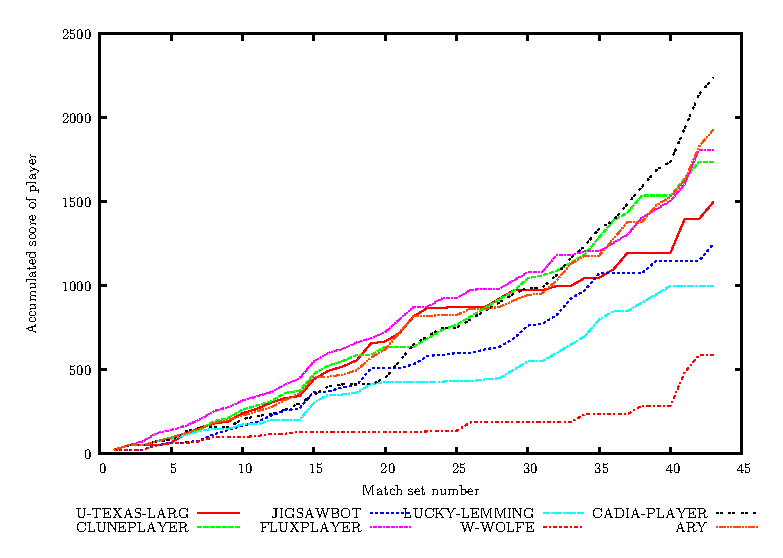
\includegraphics[width=\textwidth]{direct_scores}
 \caption{Direct scores (Competition 2007 Preliminaries; using round weights 0.25, 0.5, 0.5 and 1.0)}
 \label{fig:direct_scores}
\end{figure}

\begin{figure}
 \centering
 \includegraphics[width=\textwidth]{constant_linear_regression_1_0}
 \caption{Constant linear regression ratings (Competition 2007 Preliminaries, constant learning rate = 1.0)}
 \label{fig:constant_linear_regression}
\end{figure}

\begin{figure}
 \centering
 \includegraphics[width=\textwidth]{dynamic_linear_regression_60}
 \caption{Dynamic linear regression ratings (Competition 2007 Preliminaries, dynamic learning rate = 6.0$\dotsc$1.6)}
 \label{fig:dynamic_linear_regression}
\end{figure}

\section{Installing GgpRatingSystem}

\section{Running GgpRatingSystem}

\end{document}
